\documentclass[submit]{harvardml}

% FDV: Check all frontmatter for years, due dates, book sections, etc.
\course{CS181-S23}
\assignment{Assignment \#3}
\duedate{11:59pm EST, March 23rd, 2023}

\usepackage[OT1]{fontenc}
\usepackage[colorlinks,citecolor=blue,urlcolor=blue]{hyperref}
\usepackage[pdftex]{graphicx}
\usepackage{amsmath}
\usepackage{amssymb}
\usepackage{framed}
\usepackage{color}
\usepackage{listings}
\usepackage{enumitem}
\newenvironment{ans}{
  \begin{enumerate}
  \color{blue}
}{
  \end{enumerate}
  \color{black}
}

\DeclareMathOperator*{\mean}{\mathbb{E}}

\lstset{
  language=Python,
  basicstyle=\ttfamily,
  keywordstyle=\color{blue}\bfseries,
  commentstyle=\color{red},
  stringstyle=\color{green},
  frame=single,
  showstringspaces=false,
}

\definecolor{verbgray}{gray}{0.9}

\lstnewenvironment{csv}{%
  \lstset{backgroundcolor=\color{verbgray},
  frame=single,
  framerule=0pt,
  basicstyle=\ttfamily,
  columns=fullflexible}}{}

\begin{document}

\begin{center}
{\Large Homework 3: Bayesian Methods and Neural Networks}\\
\end{center}

\subsection*{Introduction}

This homework is about Bayesian methods and neural networks. You may want to consider the lecture notes from Feb 14th to 23rd (weeks 4 and 5). Here's an outline of the questions:

\begin{enumerate}
  \item You'll explore the Bayesian paradigm and compare it with the frequentist paradigm for the Beta-Binomial conjugate pair.
  \item You'll derive the backpropagation algorithm for a single-hidden-layer neural network for the binary classification task.
  \item You'll write some code using the PyTorch library for an image classification task.
  \item You'll consider the opportunities and limitations of ML applications and learn to anticipate possible exploits of these systems.
\end{enumerate}

As always, please start early and ask questions on Ed!

Please type your solutions after the corresponding problems using this
\LaTeX\ template, and start each problem on a new page.

Please submit the \textbf{writeup PDF to the Gradescope assignment `HW2'}. Remember to assign pages for each question.  \textbf{You must include your plots in your writeup PDF. } The supplemental files will only be checked in special cases, e.g. honor code issues, etc.

Please submit your \textbf{\LaTeX\ file and code files to the Gradescope assignment `HW2 - Supplemental'}. \\


\newpage

%%%%%%%%%%%%%%%%%%%%%%%%%%%%%%%%%%%%%%%%%%%%%
% Problem 1
%%%%%%%%%%%%%%%%%%%%%%%%%%%%%%%%%%%%%%%%%%%%%

\begin{problem}[Connecting Bayesian and Frequentist Approaches]
  
  In this question, we will gain practice with Bayesian modeling and
  compare it with the frequentist paradigm.
  
  In class, we discussed \emph{Normal-Normal conjugacy.} Now
  we will turn to \emph{Beta-Binomial conjugacy.} This model can be
  visualized in the following way.
  
  You observe a fixed number \(N\) of coin flips (either
  heads or tails) of which \(Y\) (a random variable) are heads. You assume that these are
  drawn by flipping a coin with an unknown probability \(\theta\) of
  landing heads. That is, we choose a \textbf{Binomial likelihood}
  \(Y \sim \mathrm{Bin}(N, \theta)\). The PMF of this distribution is
  given by
  
  \[
  p(Y=y) = {N \choose y} \theta^{y} (1-\theta)^{N-y}.
  \]
  
  \begin{enumerate}
  \item[1.]
    \textbf{Frequentist paradigm and MLE.} The (log) likelihood is all we
    need for frequentist inference. Derive the MLE estimate for \(\theta\)
    given the observations \(Y = y\). That is, find
    \(\arg \max_{\theta} \log p(Y = y \mid \theta)\).
  
  \item[2.]
    \textbf{Beta-Binomial conjugacy.} Under the Bayesian paradigm, we must specify a
    prior distribution for the unknown parameter \(\theta\). We choose a \textbf{Beta prior}
    \(\theta \sim \mathrm{Beta}(\alpha, \beta)\). The PDF of this
    distribution is given by
    
    \[
    p(\theta) \propto \theta^{\alpha - 1} (1-\theta)^{\beta - 1}.
    \]
    
    When the prior and posterior belong to the same distribution family, we
    call the prior-and-likelihood pair a \textbf{conjugate pair.}
    
    \begin{enumerate}
      \item Derive the mean, mode, and variance of the Beta distribution. That is, for $\theta \sim \mathrm{Beta}(\alpha, \beta)$, derive
      
      \begin{enumerate}
        \item $\mean[\theta]$. See hint. \footnote{As an alternative to taking the integral, you may want to use
        \emph{reasoning by representation.} See example 8.5.2 of the Stat 110
        textbook. If you do so, please explain the derivation in your own
        words!}
        \item $\arg \max_{\theta} p(\theta)$ when $\alpha > 1$ and $\beta > 1$. What happens otherwise? (Consider $p(0)$ and $p(1)$.)
        \item $\mathrm{Var}(\theta) = \mean[\theta^2] - (\mean[\theta])^2$.
      \end{enumerate}

      Qualitatively speaking, what does this distribution look like for different $\alpha$ and $\beta$? You can either plot this yourself or see \href{https://en.wikipedia.org/wiki/Beta_distribution}{its Wikipedia page} after deriving the statistics above. What does $\mathrm{Beta}(1, 1)$ correspond to?

      \item 
      Show that the posterior
      \(p(\theta \mid Y=y)\) is indeed Beta and derive its parameters. This proves that a Beta prior and a Binomial likelihood form a conjugate pair; in other words, the Beta distribution is a \textbf{conjugate prior} for the Binomial distribution. See hint.\footnote{For convenience in calculation: Do you need to calculate the normalizing constant? Reuse your results from the previous part.}
    \end{enumerate}
  
\end{enumerate}
\end{problem}

\newpage
\begin{framed}
\begin{enumerate}
  \item[3.]
    \textbf{Posterior mean and mode.} Often we wish to work with just a
    single point estimate of the posterior. Two commonly used point
    estimates are the \emph{posterior mean} and the \emph{posterior mode}
    (a.k.a. the maximum a posteriori (MAP) estimate).
  
    \begin{enumerate}
    \item
      Discuss the advantages and disadvantages of using posterior point
      estimates. Which of these are relevant for our Beta-Binomial conjugate pair? Consider the case when $\alpha, \beta < 1$.
    
    \item
      Using your results from part 2, write down
      
      \begin{enumerate}
        \item the posterior mean estimate \(\theta_{\text{post mean}} = \mean [\theta \mid Y = y]\),
        \item the posterior MAP estimate \(\theta_{\text{MAP}}=\arg \max_{\theta}p(\theta \mid Y=y)\),
        \item and the posterior variance $\mathrm{Var}(\theta \mid Y = y) = \mean[\theta^2 \mid Y = y] - (\mean[\theta \mid Y = y])^2$.
      \end{enumerate}
      
      You shouldn't need any further derivations. That's the nice thing about conjugate priors!
      
    \end{enumerate}

\item[4.]
    \textbf{Prior-posterior connections.}

    \begin{enumerate}
    \item
      Explain in your own words how \(\alpha\) and \(\beta\) affect the
      MAP estimate. How would you set \(\alpha\) and \(\beta\) to reflect
      a prior belief that the coin is fair (i.e.~shows heads and tails
      with equal probability)? (Be careful! See 2.a.ii.)

    \item Now let's analyze the variances of our prior and posterior distributions. Consider the case when $\alpha = \beta$. (If you'd enjoy it, consider the general case for a better understanding.) A sentence or two for each point is fine.
    \begin{enumerate}
      \item How does the variance of the prior relate to the variance of the posterior?
      \item How might you use the prior variance to encode a stronger or weaker prior belief?
      \item How does the posterior variance change as we observe more samples $n$?
    \end{enumerate}
    \end{enumerate}

  \item[5.]
    \textbf{Analysis and connection to frequentism.}
  
    \begin{enumerate}
    \item
      Write a loss function \(\ell(\theta) \in \mathbb{R}\) in terms of
      \(\theta, y, n, \alpha, \beta\) such that minimizing \(\ell\) is
      equivalent to calculating the MAP estimate,
      i.e.~\(\theta_{\text{MAP}} = \arg \min_{\theta} \ell(\theta)\). Your
      function should be a sum of:
      \begin{enumerate}
        \item a mean-squared-error term (which should loosely resemble $(y - \hat y)^2$)
        \item a
        regularization term \(g(\theta) = - a \theta + b \theta^{2}\) for some $a, b$.
      \end{enumerate}
      
      Can you interpret the regularization term? 
      
      Hint: Work backwards from part 1 to derive the MSE term and from part 2.a.ii to get the regularization term. Watch out for the signs! For the interpretation, complete the square and then compare your expression with the prior mode you found in 2.a.ii.
    \item
      What happens to both $\theta_{\text{post mean}}$ and $\theta_{\text{MAP}}$ as \(n \to \infty\)? Compare this to the MLE estimate.
      (Remember to account for the change in \(y\).)
    \end{enumerate}
  
\end{enumerate}

\end{framed}

\subsection*{Solution:}

\newpage
\begin{ans}
    \item We first find the likelihood function. We can drop the binomial coefficient since it is a constant, and we get 
    $$
    L(\theta;  Y) = \theta^{y}(1 - \theta)^{N -y}
    $$
    The log of this is 
    $$
    \ell (\theta;  Y) = y \log \theta + N \log (1 - \theta) - y\log (1 - \theta)
    $$
    Taking the derivative w.r.t. $y$, we get
    $$
    s (\theta;  Y) = y/\theta - N / (1 - \theta) + y/ (1 - \theta) = 0 \implies \hat \theta _{MLE} = y/N
    $$
    \item  
        \begin{enumerate} 
        \item
        \begin{enumerate}
            \item To find the mean, we can use the Bank-Post Office result, as outlined on page 397 of the Stat 110 Book. First, consider some Beta variable $W$ such that $W = \frac{X}{X + Y}$, where $X \sim \text{Gamma}(a, \lambda)$ and $Y \sim \text{Gamma}(b, \lambda)$. Then, by definition, 
            $$
            \mean[W] = \mean [\frac{X}{X + Y}]
            $$
            By the Bank-Post Office Result, we first define another variable: $T = X + Y$. We can use this result to say that $\mean[TW] = \mean[T]\mean[W]$. Therefore, plugging in, we have 
            $$
            \mean \left[(X + Y) \frac{X}{X + Y}\right] = \mean [(X + Y)]\mean \left[\frac{X}{X + Y}\right]
            $$
            Simplifying, and applying the Bank-Post Office result again toward the independence of $X + Y$ and $X$, we have
            $$
            \mean \left[\frac{X}{X + Y}\right] = \frac{\mean [X]}{\mean[X + Y]}
            $$
            Now, plugging in for the expectation of Gamma variables and simplifying, we have
            $$
            \mean [W] = \frac{a}{a + b}
            $$
            
            
            \item I drop $n \choose k$ here since it's a constant. $q = 1 - p$
            $$
            P(Y = k) =& {n \choose k}\int_{p = 0}^1 P(X = k | p)f(p) dp 
            $$
            $$
            &=  \int_{p = 0}^1 p^{\alpha + k - 1} q^{\beta + n - k - 1} dp
            $$
            In this step, I combine the terms in the PDFs of beta and binomial and also then drop constants: $\frac{1}{\beta (\alpha, \beta)}$ and $n \choose k$. Therefore, if this is our PDF, we can pattern-match to the beta function and get this for our posterior likelihood:
            $$
            L(p ; Y = k) = \text{Beta}(\alpha + k, \beta + n - k)
            $$
            To maximize this, we note that we maximize $p(\theta)$ by taking the log's derivative, setting it to zero, and verifying that $p$ is globally concave. (We can maximize the log and get the same point because it is monotonic increasing.)
        $$
        \log p(\theta) = (\alpha - 1) \log\theta + (\beta - 1)\log(1 - \theta) \implies \frac{(\alpha - 1)}{\theta} + \frac{1 - \beta}{1 - \theta} = 0
        $$
        Doing this, we get the following result
        $$
        \frac{1-\alpha}{2 - \beta - \alpha}
        $$
        This is globally concave:
        $$
        \frac{\partial ^2}{\partial^2 \theta} = \frac{(1 - \alpha)}{\theta^2} + \frac{1 - \beta}{(1 - \theta)^2}
        $$
        The above will always be less than or equal to zero because the first term's numerator will be negative since $\alpha > 1$, and its denominator will be nonnegative; and the second term will always be negative for the same reason. 
        If $\alpha$ or $\beta < 1$, then we can get a divide by zero error (and if they are greater than one, we can't) or, we can get a bimodal distribution, so there might not exist only one mode, or the mean could return a useless answer because it will be in a valley between the two modes, i.e., a region where the estimate is actually quite unlikely, on our priors. 
        \item To find variance, we first find $\mean [\theta^2]$, which we can do by integrating over the PDF:
        $$
        \int_{0}^1 \theta^2 (\theta^{\alpha - 1}(1-\theta)^{\beta - 1}) d\theta = \frac{1}{\alpha + 2} - \frac{1}{\alpha + \beta + 1}
        $$
        Therefore, using the definition of variance, we have
        $$
        \mean[\theta^2] - \mean[\theta]^2 = \frac{1}{\alpha + 1} - \frac{1}{\alpha + \beta + 1} - \frac{\alpha^2}{(\alpha + \beta)^2}
        $$
        If we let $\mu = \frac{\alpha}{\alpha + \beta}$, then we have variance of 
        $$
        \frac{\mu(1 - \mu)}{\alpha + \beta + 1}
        $$
        \end{enumerate}
        Beta(1, 1) corresponds to a Uniform distribution from 0 to 1. If we scale $\alpha$ and $\beta$, very informally, we get that lower $\alpha$ makes the distribution have a higher PDF value towards the left and higher $\beta$ makes it have higher PDF values towards the right. Higher values for both correspond to a more hump-shaped/normal-looking distribution, and lower values for both mean the distribution is more U-shaped (i.e., the PDF has higher value near to 0 and 1). Finally, higher values for either correspond to steeper curves. 
        \item We can verify Beta-Binomial Conjugacy by plugging in for the posterior, which is proportional to likelihood times prior:
        $$
        (\theta^y(1 - \theta)^{N - y}) \cdot (\theta^{\alpha - 1}(1 - \theta)^{\beta - 1}) = \theta(y + \alpha - 1)(1 - \theta)^{\beta + N - y - 1}
        $$
        Thus, we can pattern-match this to a Beta$(y + \alpha, \beta + N - y)$ distribution.         
    \end{enumerate}
    \item
    \begin{enumerate}
        \item Posterior point estimates can be useful in that they condense our distribution down to a single number, which is useful in that we can make point predictions from single number, but we cannot make point predictions from distributions; we can make distributions of predictions. However, condensing a distribution down to a point also destroys information and can be misrepresentative (for example, as discussed in class, if we have a bimodal posterior and take the MAP, we will end up discarding a large portion of the data from the posterior because we will neglect one of the modes). We care about the following point estimates: mean and mode. 
        % !! What do I say about a|| b < 1? 
        When $\alpha < 1$ or $ \beta < 1$, our mean and mode estimates become much less useful. In this case, when both are less than one, the distribution becomes u-shaped, so the mean will be in between the peaks; i.e., in a very low-probability region; and there will be potentially multiple peaks with the same value, so we cannot return one mode (there will be two), in the case $\alpha = \beta$. Otherwise, we will be able to return a mode, but it will not capture the information fully because we will neglect the other mode. 
        \item Using the results from above, 
        \begin{enumerate}
            \item $\mean \theta_\text{post} = \frac{y + \alpha}{y + \alpha + \beta + N - y}$
            % \item $\theta_\text{MAP} = \frac{(1 - y - \alpha)}{\theta^2} + \frac{1 - \beta - N + y}{(1 - \theta)^2}$
            \item $\theta_{\text{MAP}} = \frac{y + \alpha - 1}{n + \alpha + \beta - 2}$
            \item If we let $\mu$ be the result in i), then $\text{Var}(\theta | Y = y) = \frac{\mu(1 - \mu)}{y + \alpha + \beta + N - y + 1}$
        \end{enumerate}
    \end{enumerate}
    \item 
    \begin{enumerate}
        \item The prior distribution will pull the MAP toward the prior mean--i.e., if we have a prior centered on 0.5, then the MAP will be more likely to be near 0.5. Put another way, higher $\alpha$ means we think the probability is more likely to be low, and higher $\beta$ means we think it is more likely to be high. High values for both tightens the distribution. Therefore, if I thought a coin was probably fair, I would set high values for both $\alpha$ and $\beta$. This produces a distribution where the mean is near $0.5$. 
        \item 
        \begin{enumerate}
            \item Assuming constant variance in the data, they are positively correlated. 
            \item I would decrease the variance in the prior to encode a stronger belief (for example, a distribution with a large hump at $0.5$ if I thought a coin was probably fair). 
            \item It decreases because the likelihood for different values decreases the least around the true value, so the posterior distribution tightens around the true value. 
        \end{enumerate}
    \end{enumerate}
    % \item From Derivation 2.9.1 in the book, consider likelihood function 
    \item 
    \begin{enumerate}
        \item 
    We have already derived the MAP estimate, and we know that this estimate comes from the loss function $\ell$ where setting $\ell'(\theta) = 0 \implies \theta = \theta_{\text{MAP}}$. Therefore, we can take our result from above and set it equal to zero:
    $$
    \frac{y + \alpha - 1}{n + \alpha + \beta - 2} = \theta_{\text{MAP}} \equiv \frac{y + \alpha - 1}{n + \alpha + \beta - 2} - \theta_{\text{MAP}} = 0
    $$
    We know that our loss function is of the form 
    $$
    c(y - n\theta)^2 - a\theta + b\theta^2
    $$
    So we can take the derivative of this and pattern-match it with our MAP estimate:
    $$
    \frac{d}{d\theta} c(y - n\theta)^2 - a\theta + b\theta^2 = -2c(y - n\theta) - a + 2b\theta  = 0
    $$
    Now, we solve for $\theta$, and get that
    $$
    -2cy + 2cn\theta - a + 2b\theta \implies \theta_{\text{MAP}} = \frac{2cny + a}{2cn^2 + 2b} = \frac{\alpha + y - 1}{\alpha + \beta + n - 2}
    $$
    Therefore, solving for these constants, we get 
    $$
    a = \alpha - 1, b = \frac{\alpha + \beta}{2} - 1, c = \frac{1}{2n}
    $$
    I.e., 
    $$
    \frac{1}{2n}(y - n\theta)^2 - (\alpha - 1)\theta + (\frac{\alpha + \beta}{2} - 1)\theta^2
    $$
    Interpreting this, we complete the square on the regularization term and get 
    $$
    \frac{\alpha + \beta - 2}{2}\left(\theta - \frac{\alpha - 1}{\alpha + \beta - 2}\right)^2
    $$
    We can pattern-match $\frac{\alpha - 1}{\alpha + \beta - 2}$ to the mean of our prior, which makes sense: this is saying the results will get pulled toward the mean of our prior. 
    \item Both go to $\frac{y}{n}$: if we look at our expressions, we have 
    $$
    \frac{1-\alpha}{2 - \beta - \alpha} = \theta_{\text{MAP}}
    $$
    and 
    $$
    \frac{\alpha + y}{\beta + n + \alpha}
    $$
    Remember $y$ is distributed such that $\mean [Y] = n \theta$ and $\text{Var}(Y)=\frac{\sigma^2}{n}$. Therefore, as $n \to \infty$, our other constants $\alpha, \beta, 2,$ and $1$ will become less and less significant and we will be left with expressions asymptotically equivalent to 
    $$
    \frac{y}{n} = \frac{n\theta}{n} = \theta
    $$
    ($\frac{Y}{n} = \bar Y \to \theta$ is also true by LLN.)
    \end{enumerate}
    \end{ans}
\newpage


\newpage

%%%%%%%%%%%%%%%%%%%%%%%%%%%%%%%%%%%%%%%%%%%%%
% Problem 2
%%%%%%%%%%%%%%%%%%%%%%%%%%%%%%%%%%%%%%%%%%%%%

\begin{problem}[Neural Networks]

    In this problem, we will take a closer look at how gradients are calculated for backprop with a simple multi-layer perceptron (MLP). The MLP will consist of a first fully connected layer with a sigmoid activation, followed by a one-dimensional, second fully connected layer with a sigmoid activation to get a prediction for a binary classification problem. We use non-linear activation functions as the composition of linear functions is linear. Assume bias has not been merged. Let:
    \begin{itemize}
        \item $\bold{W}_1$ be the weights of the first layer, $\bold{b}_1$ be the bias of the first layer.
        \item $\bold{W}_2$ be the weights of the second layer, $\bold{b}_2$ be the bias of the second layer.
    \end{itemize}
    
    The described architecture can be written mathematically as: $$\hat{y} = \sigma(\bold{W}_2 \left[\sigma \left(\bold{W}_1 \bold{x} + \bold{b}_1\right)\right] + \bold{b}_2)$$
    
    where $\hat{y}$ is a scalar output of the net when passing in the single datapoint $\bold{x}$ (represented as a column vector), the additions are element wise additions, and the sigmoid is an element wise sigmoid.
    
    \begin{enumerate}
        \item Let:
        \begin{itemize}
            \item $N$ be the number of datapoints we have
            \item $M$ be the dimensionality of the data
            \item $H$ be the size of the hidden dimension of the first layer. Here, hidden dimension is used to describe the dimension of the resulting value after going through the layer. Based on the problem description, the hidden dimension of the second layer should be 1.
        \end{itemize}
        
        Write out the dimensionality of each of the parameters, and of the intermediate variables:
  
            \begin{align*}
            \bold{a}_1 &= \bold{W}_1 \bold{x} + \bold{b}_1, 
            &\bold{z}_1 = \sigma(\bold{a}_1) \\
            a_2 &= \bold{W}_2 \bold{z}_1 + \bold{b}_2, 
            &\hat{y} = z_2 = \sigma(a_2)
            \end{align*}
            
        and make sure they work with the mathematical operations described above. Examining shapes is one of the key ways to debug your code, and can be done using .shape after any numpy array.
        
        \item  We will derive the gradients for each of the parameters, which can then be used along with gradient descent to find weights that improve our model's performance. For this question, assume there is only one datapoint $\bold{x}$, and that our loss is $L = -(y \log (\hat{y}) + (1 - y) \log (1 - \hat{y}))$. For all questions, the chain rule will be useful.
      \begin{enumerate}
          \item Find $\frac{\partial L}{\partial b_2}$. 
          
          \item Find $\frac{\partial L}{\partial W_2^h}$, where $W_2^h$ represents the $h$th element of $\bold{W}_2$.
          
          \item Find $\frac{\partial L}{\partial b_1^h}$, where $b_1^h$ represents the $h$th element of $\bold{b}_1$. (*Hint: Note that only the $h$th element of $\bold{a}_1$ and $\bold{z}_1$ depend on $b_1^h$ - this should help you with how to use the chain rule.)
          
          \item Find $\frac{\partial L}{\partial W_1^{h,m}}$, where  $W_1^{h,m}$ represents the element in row $h$, column $m$ in $\bold{W}_1$.
      
      \end{enumerate}

\end{enumerate}

\end{problem}
\newpage
\newpage 

\begin{framed}
    \noindent\textbf{Problem 2} (cont.)\\
    \begin{enumerate}
    \setcounter{enumi}{2}
    
      \item  We now explore an example of forward-mode auto-differentiation. Consider the following 
          equation:
          $$
            f(x_1, x_2) = \ln (\sin (x_1)) + x_1 \exp \{ x_2 \}
          $$
    
          This equation can be split up using intermediate variables $v_1, \dots, v_7$ as follows:
    
          \begin{align*}
            v_1 &= x_1 \\ 
            v_2 &= \sin (v_1) \\
            v_3 &= \ln (v_2) \\
            v_4 &= x_2 \\
            v_5 &= \exp \{ v_4 \} \\
            v_6 &= v_1v_5 \\
            v_7 &= v_3 + v_6 \\
            f(x_1, x_2) &= v_7
          \end{align*}
    
            Splitting up the equation like this is very similar to what an auto-differentiation 
            library would do. From these equations we can construct a \textit{computational graph} 
            where each node of the graph corresponds to an input, an intermediate variable, or 
            the output. 
    
        \begin{enumerate}
            \item Let $x_1 = \frac{\pi}{6}$ and $x_2 = 1$. Calculate the values of all the 
                intermediate variables $v_1, \dots v_7$ and $f(x_1,x_2)$. 
            \item Calculate the derivative of
                all of the intermediate variables $v_1, \dots, v_7$ and
                $f$ with respect to $x_1$ evaluated 
                at $x_1 = \frac{\pi}{6}$ and $x_2 = 1$.  
    
        \end{enumerate}
    
    \item \textbf{Extra Credit (Hard):} Consider two neural networks $f_1$ and $f_2$ for binary 
        classification. They each take in inputs $x \in \mathbb{R}^2$ and output a 
        prediction $\hat{y} \in [0,1]$. $f_1$
        consists of a single hidden layer with 4 nodes, each with 
        a ReLU activation function. These nodes are connected to a single sigmoid output node. Thus 
        $f_1$ has the following form:
    
        $$
        f_1(x) = \sigma\left( W_2[ReLU(W_1 x + b_1)] + b_2 \right)
        $$
    
        $f_2$ consists of 2 hidden layers, each with 2 ReLU activated nodes. Just as in $f_1$, the 
        nodes of the final layer are connected to a single sigmoid output node. 
        Thus $f_2$ has the following form:
    
        $$
        f_2(x) = \sigma(W_3[ReLU(W_2[ReLU(W_1 x + b_1)]+b_2)]+ b_3)
        $$
    
        We leave finding the shapes of the weight and bias vectors up to you, noting that 
        by convention $x$ should be considered a column vector with 2 elements. 
    
        Draw a classification boundary that $f_2$ can express but $f_1$ cannot and argue 
        why $f_2$ can express the boundary but $f_1$ cannot.
    
    
    \end{enumerate}  
\end{framed}

\subsection*{Solution:}

\begin{ans}
    \item 
    % How much justification?
    \begin{enumerate}
        \item $\mathbf x$ is of shape $M \times 1$ because we have one datapoint, so we have one row. 
        % \item $\mathbf W_1$ is of shape $H \times 1$ since it takes $\mathbf x$ as its input, and by definition outputs to the first hidden layer. This implies that $\mathbf b_1$ and $\mathbf a_1$, and $\mathbf z_1$ are of shape $H \times 1$
        \item $\mathbf W_1$ is of shape $H \times M$ since it takes $\mathbf x$ as its input, and by definition outputs to the first hidden layer. This implies that $\mathbf b_1$ and $\mathbf a_1$, and $\mathbf z_1$ are of shape $H \times 1$
        \item $\mathbf W_2$ is of shape $1 \times H$ because it takes the $H \times 1$ input from the previous step and we want an output of shape $1 \times 1$. 
        Therefore, $\mathbf b_2$, $a_2$, and $z_2$ are of shape $1 \times 1$
    \end{enumerate}
    \item 
    \begin{enumerate}
        \item We can find this via the Chain Rule:
        $$
        \frac{\partial L}{\partial \mathbf b_2} = \frac{\partial L}{\partial \hat y}\frac{\partial \hat y}{\partial a_2} \frac{\partial a_2}{\partial \mathbf b_2} = \left(\frac{1 - y}{1 - \hat y}-\frac{y}{\hat y}\right) \left((1 - \sigma(a_2)) \sigma(a_2)\right) \cdot 1
        $$
        \item We get the following from the Chain Rule:
        $$
        \frac{\partial L}{\partial W_2^h} = \frac{\partial L}{\partial \hat y}\frac{\partial \hat y}{\partial \mathbf W_2^h}=\left(\frac{1 - y}{1 - \hat y}-\frac{y}{\hat y}\right) \sigma(a_2)(1 - \sigma(a_2))\mathbf z_1^h
        $$
        $ \mathbf z_1^h$ comes from the fact that, recalling part 1, we have a $1 \times H$ matrix, $\mathbf W_2$, times an $H \times 1$ matrix. This is mathematically equivalent to $\sum_{j = 1}^H W_2^j z_1^j$; therefore, we can just take the derivative of the $h$th term of this sum, which is $z_1^j$. 
        \item Chain Rule gives:
        $$
        \frac{\partial L}{\partial b_1^h} = \frac{\partial L}{\partial \hat y} \frac{\partial \hat y}{\partial a_2^h} \frac{\partial a_2^h}{\partial z_1^h}\frac{\partial z_2^h}{\partial a_1^h}\frac{a_1^h}{b_1^h}
        $$
        Plugging in, we have
        $$
        (\frac{1 - y}{1 - \hat y}-\frac{y}{\hat y}) \cdot \sigma(a_2)(1 - \sigma(a_2))\cdot W_2^{1, h} \cdot\sigma(a_1^h)(1 - \sigma(a_1^h))
        $$
        \item By Chain Rule,
        $$
         \frac{\partial L}{\partial W_1^{h, m}} = \frac{\partial L}{\partial \hat y} \frac{\partial \hat y}{\partial a_2} \frac{\partial a_2}{\partial z_1^h}\frac{\partial z_1^h}{\partial a_1^h}\frac{a_1^h}{W_1^{h, m}}
        $$
        We have
        $$
        = (\frac{1 - y}{1 - \hat y}-\frac{y}{\hat y}) \cdot \sigma(a_2)(1 - \sigma(a_2)) \cdot W_2^{1, h}\cdot \sigma(a_1^h)(1-\sigma(a_1^{h})\cdot X_{m, 1}
        $$
    \end{enumerate}
    \item
    \begin{enumerate}
    \item The values are as follows:
    \newline
     \begin{enumerate}
        \item $v_1 = \frac{\pi}{6}$
        \item $v_2 = 1/2$
        \item $v_3 = -\ln 2$
        \item $v_4 = 1$
        \item $v_5 = e$
        \item $v_6 = \frac{e\pi}{6}$
        \item $v_7 = -\ln 2 $
    \end{enumerate}
    \newpage
    \item 
    \begin{tabular}{|c|c|c|}
        \hline
        $i$ value & $\frac{\partial v_i}{x_1}$ & $\frac{\partial v_i}{x_2}$ \\
        \hline
        1 & 1 & 0 \\
        2 & $\cos(x_1) = \cos\frac{\pi}{6}$ & 0 \\
        3 & $\frac{1}{\sin(v_1)}\cos(x_1) = \sqrt 3$ & $0$\\
        4 & 0 & 1 \\
        5 & 0 & $e$ \\ 
        6 & $e^{x_2}$ & $x_1e^{x_2}$ \\ 
        7 & $\sqrt 3 + e^{x_2}$ & $0 + x_1e^{x_2}$\\
        \hline
    
        \end{tabular}
    \end{enumerate}
\end{ans}

\newpage

%%%%%%%%%%%%%%%%%%%%%%%%%%%%%%%%%%%%%%%%%%%%%
% Problem 3
%%%%%%%%%%%%%%%%%%%%%%%%%%%%%%%%%%%%%%%%%%%%%

\begin{problem}[Modern Deep Learning Tools: PyTorch]

In this problem, you will learn how to use PyTorch. This machine learning library is massively popular and used heavily throughout industry and research. 


\begin{enumerate}
    \item In \verb|T3_P3.ipynb| you will implement an MLP for image classification from scratch. Paste your code solutions below and include a final graph of your training progress. Also submit your completed \verb|T3_P3.ipynb| file.
    \item Discuss what trends you see with your plot (train/test loss and train/test accuracy).
\end{enumerate}

\textbf{Out of Distribution (OOD) Analysis}: Now, let's evaluate the usefulness of the predictive uncertainties of our model for test data that are dissimilar to our training data. These test data points are called out of distribution (OOD) points. Just as in Homework 2, we want the predictive uncertainties from our models to help us distinguish in-distribution test data (test data that are similar to data on which we trained our model) and OOD test data. Again, in many safety-critical applications of ML, we want human-experts to override model decisions if the model is operating on extremely unfamiliar data. 

\hspace{3mm} 3. Report both the in and out distribution test accuracies of your model. In a couple of sentences, discuss what you notice about these accuracies.

  {\bfseries You will recieve no points for code not included below.}

  {\bfseries You will recieve no points for code using built-in APIs from the \verb|torch.nn| library.}
  
\end{problem}


\subsection*{Solution:}

Plot:

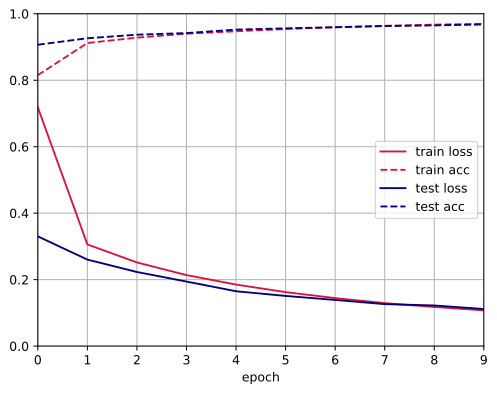
\includegraphics[width=\linewidth]{hw3/ML plot.png}

Code:

\begin{lstlisting}[language=Python]
J = 256
# mini-batch size = 4
M = 4
# flatten 28 * 28 image into a row vector of length 28 * 28
D = 28 * 28
K = 10

W1 = torch.nn.Parameter(0.01 * torch.randn(size=(D, J))) # matrix applying linear transformation
b1 = torch.nn.Parameter(0.01 * torch.randn(size=(1, J))) # additive bias term
W2 = torch.nn.Parameter(0.01 * torch.randn(size=(J, K))) # matrix applying linear transformation
b2 = torch.nn.Parameter(0.01 * torch.randn(size=(1, K))) # additive bias term

W1.requires_grad = True
b1.requires_grad = True
W2.requires_grad = True
b2.requires_grad = True

params = [W1, b1, W2, b2]


def relu(x):
  return torch.clamp(x, min=0)

def softmax(x):
  return torch.exp(X) / torch.sum(torch.exp(X), dim=1, keepdim=True)


def net(X):
  X = X.view(-1, D)
  
  A1 = X @ W1 + b1
  H = relu(A1)
  A2 = H @ W2
  Z2 = A2 + b2
  y_hat = softmax(Z2)
  return y_hat


def cross_entropy(y_hat, y):
  y_onehot = torch.zeros(y_hat.shape)
  y_onehot.scatter_(1, y.view(-1, 1), 1)
  return -torch.sum(y_onehot * torch.log(y_hat), dim=1)



def sgd(params, lr=0.1):
  with torch.no_grad():
    for param in params:
      param -= lr * param.grad
      param.grad.zero_()


def train(net, params, train_iter, loss_func=cross_entropy, updater=sgd):
  for epoch in range(10):
    total_loss = 0
    for X, y in train_iter:
      y_hat = net(X)
      total_loss += loss_func(y_hat, y)
      avg_loss = total_loss / M
      avg_loss.backward()
      updater(params)
\end{lstlisting}
\begin{ans}
    \item See above
    \item In the plot 
    \begin{enumerate}
        \item As we would expect, train accuracy becomes greater than test accuracy by the end of the test as the model gets fit on train data, even though at the beginning, the test accuracy is actually better!
        \item Train and test loss/accuracy get better in smaller and smaller steps, which makes sense, as it matches up with how we would expect the surface we're performing gradient descent on to look (i.e., generally with nonzero Hessian). 
    \end{enumerate}
    \item I got in-distribution accuracy of 0.9963235294117647 and out-of-distribution accuracy of 0.4339706599712372. This suggests that the model is overfit: obviously, $\approx 99\%$ accuracy is nearly perfect. If our model was well-fit, we would expect out-of-distribution accuracy above, say, $80\%$ ("reasonably good"). $40\%$ is not in the same region of accuracy. 
\end{ans}
\newpage

%%%%%%%%%%%%%%%%%%%%%%%%%%%%%%%%%%%%%%%%%%%%%
% Problem 4
%%%%%%%%%%%%%%%%%%%%%%%%%%%%%%%%%%%%%%%%%%%%%

\begin{problem}[Impact Question: Testing security of neural networks deployed in autonomous vehicles and suggesting policy recommendations (9 points)]

\textbf{The learning goal of the impact questions of this homework is
three-fold: }

\begin{enumerate}
\item
  Get trained in adversarial thinking to be able to anticipate risks and
  possible exploits when designing Machine Learning applications
\item
  Understand opportunities and limitations to safety and security of
  Machine Learning applications
\item
  Learn to put yourself in the shoes of policymakers who are in charge
  of ensuring safety of real-world Machine Learning applications.
\end{enumerate}

\textbf{Prompt: }You are the Director of Machine Learning of the US
Department of Transportation (a federal US government agency).

The Secretary of the US Department of Transportation declares security
of Machine Learning applications deployed in autonomous vehicles as one
of the priorities of the agency. You are tasked to assess the security
of Machine Learning systems deployed in autonomous vehicles and develop
policy recommendations for the US Department of Transportation.

\textbf{Context: }Tesla employs Neural Networks for perception and
control tasks: For example semantic segmentation, object detection and
monocular depth estimation is performed by Neural Networks on images
captured with the car's camera system to identify road signs, traffic
lights, pedestrians, cars or other traffic related individuals,
vehicles, and objects. The full build autopilot consists of more than 48
networks which must identify high-risk scenarios and provide robust
predictions to ensure safety.

Moreover, beyond cameras Tesla also uses additional sensor systems such
as LiDAR or ultrasonic sensors. Yet, Tesla's engineering and design
approaches are still iterated and their software gets updated.

Link to a demo video: \url{https://tesla-cdn.thron.com/static/NGSLYL_network_XZCUMR.mp4}

Please answer the questions below by using concise language (350 - 700
words in total). Bullet points are appropriate.

\textbf{Questions: }

\begin{enumerate}
\item
  \textbf{Adversarial thinking: }List and explain 3 options how you
  could attack the Neural Network deployed in a self-driving car to make
  it crash. In particular, explain the impact of the attack on the
  statistical properties of input data and predictions of the Neural
  Network. (3 points)

  \begin{enumerate}
  \item
    \textbf{Hardware adversarial attack: }List and explain one attack
    which targets the hardware system of an autonomous vehicle or its
    physical surround.
  \item
    \textbf{Software adversarial attack:} List and explain one attack
    which targets the software system of an autonomous vehicle.
  \item
    \textbf{Social engineering:} List and explain one attack which
    relies on social engineering to make an autonomous vehicle crash.
  \end{enumerate}

\item
  \textbf{Safeguards: }For each of the 3 attack options that you listed
  above, suggest and explain one possible solution that could safeguard
  the Neural Network deployed in Tesla's autopilot. (3 points)

\item
  \textbf{Policy recommendation: }The Secretary of the US Department of
  Transportation asks you to develop one policy recommendation on how to
  ensure sufficient security of deployed neural networks in autonomous
  vehicles.

  \begin{enumerate}
  \item
    \textbf{Recommendation:} List and explain one policy recommendation
    that the US Department of Transportation should implement. (1 point)
  \item
    \textbf{Benefit: }List and explain one benefit of your chosen
    recommendation. (1 point)
  \item
    \textbf{Drawback: }List and explain one drawback of your chosen
    recommendation. (1 point)
  \end{enumerate}
\end{enumerate}

\end{problem}

\newpage

\subsection*{Solution:}
\begin{ans}
    \item 
    \begin{enumerate}
        \item One adversarial attack in the hardware is, if the camera/LiDAR/perception systems aren’t sufficiently redundant and the car doesn’t have sufficient alert systems, an adversary could break or disable the sensors and prevent them from working. E.g., he could put duct tape on the cameras. 
        \item A hack could target the software side of the system. For example, a Man in the Middle attack could intercept database connections and impersonate http responses (I know there have already been several instances of hacking cars' computer systems, so it seems like a reasonable extension to add this capability to the self-driving aspect). 
        \item A phishing attack could consist of an email pretending to be a software update to be installed on the self-driving capabilities, but actually be one that either steals the drivers information or causes the car to crash. 
    \end{enumerate}
    \item \begin{enumerate}
        \item Mandating some sort of detection system to alert the driver when sensors are broken or compromised would prevent against this. With this safeguard, the car could not activate self-driving capabilities without service, preventing the compromised sensors from leading the system to make poor driving decisions. 
        \item The best fix for this is to make more secure software systems and communication protocols using, for example, encryption. 
        \item The manufacturer could make the car's software closed-source, preventing consumers from installing additions onto it. To lower the likelihood of this kind of information phishing, manufacturers could make especially clear to the consumer how they will communicate with them, thus implying that other methods will be phishers
    \end{enumerate}
    \item \begin{enumerate}
        \item \textbf{Policy}: it seems like the avenues with the highest potential for hacking are via internet connections (this is what a report by the European Union Agency for Cybersecurity found), and the other vulnerabilities I listed above are likely enough and low-cost enough that we can expect the free market to adequately embed incentives for interventions addressing these vulnerabilities. I am no cybersecurity expert, but I would mandate some sort of internet connection "containerization" - i.e., the self-driving systems have to somehow insulate their self-driving decision-making apparati from from real-time data received over an internet connection. 
        \begin{enumerate}
            \item One specific requirement toward this end is to mandate virtualization technology to create isolated environments for the self-driving decision-making apparatus. In this approach, the self-driving decision-making software would run in a virtual machine (VM) that is isolated from the rest of the system and the Internet
            \item Another potential approach would be to mandate any connections to external sources are encrypted, ensuring the data is authentic. I lean toward this requirement because it seems reasonably low-cost and high-benefit to implement, and is something that you build on top of the software, rather than something you have to build the software around. 
        \end{enumerate}
        \item \textbf{Benefit}: We have seen relatively few phishing attacks of this kind, but, in the likely event they become more common, this would be a high-benefit intervention: it could save the lives of drivers whose cars would have otherwise been easily hacked. 
        \item \textbf{Cost}: Generally, we should be hesitant about regulating continuously-evolving technology: government can have a poor track record at this: often, they mandate that a solution must match overly-restricting criteria, and, in doing so, preclude some better solution that was unknown when the policy was implemented. Given the evolving nature of self-driving technology, I suspect this might be one of these cases. 
    \end{enumerate}
\end{ans}
\

\newpage

%%%%%%%%%%%%%%%%%%%%%%%%%%%%%%%%%%%%%%%%%%%%%
% Name and Calibration
%%%%%%%%%%%%%%%%%%%%%%%%%%%%%%%%%%%%%%%%%%%%%
\subsection*{Name}

\subsection*{Collaborators and Resources}
Whom did you work with, and did you use any resources beyond cs181-textbook and your notes?

\href{https://www.lifewire.com/how-self-driving-cars-can-be-hacked-5114337}{EU Cybersecurity Study}

\subsection*{Calibration}
Approximately how long did this homework take you to complete (in hours)? 


\end{document}
